\section{Game Changers} \label{game_changers}

\emad{As discussed, we should merge this with trendds. Once you do that, I will have a look at the trends section again.}
%%%%%%%%%%%%
% Perceived Quality
% Software is more than just developing code
% Software intelligence can bridge both worlds.

\revised{Section \ref{trends} reflected on our accomplishments of software defect prediction studies since the 2000s. In this section, we discuss the game changers that pursed the accomplishments and had a significant impact on software defect prediction.}

%%%%%%%%%%%%%%%%%%%%%%%%%%%%%%%%%%%%%%%%%%%%%%%%%%%%%%%%%%%
\subsection{Data}
\smallsection{OSS projects} 
Open Source Initiative, which was founded in 1998 and is an organization to dedicate to promoting open source software, describes \emph{open source software is software that can be freely used, changed, and shared (in modified or unmodified form) by anyone.}~\cite{OSI}
Nowadays, there are no end of active open source software projects online supported by a huge range of people.

An OSS project is a change changer, because it opens the development history of long-lived widely-deployed software systems.
Figure \ref{fig:oss} shows that the number of papers using OSS projects is growing over time~\cite{Shihab2012PhD}. 

Other way to access such rich data source is to cooperate with commercial organization (e.g., ABB Inc,~\cite{Li2006} and Avaya~\cite{Mockus2010FSE}).
However, commercial organization in many cases is not willing to give access to the detail of its rich data source due to confidential reasons.
While another way is to use academic projects (e.g., course projects), such projects are relatively not rich comparing with commercial projects.
In short, OSS projects provide rich, extensive, and readily available software repositories. 

%\para{Why are OSS projects a game changer? Because we can get long-lived development projects quickly.} 


%-----------------------------------------------------------------------
\begin{figure}
  \centering
  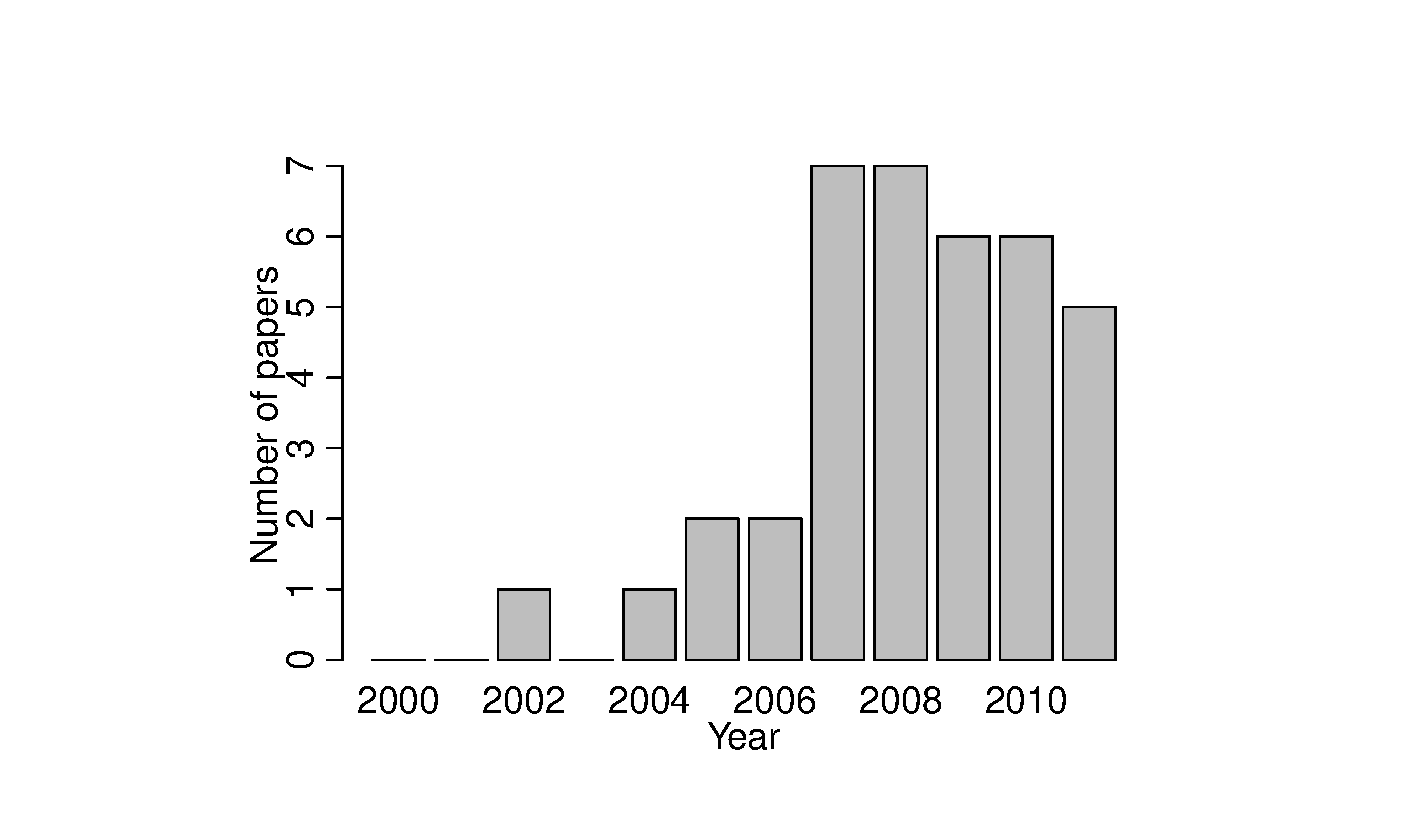
\includegraphics[trim=100 30 100 0, scale=0.5,clip]{figures/papers}
  \caption{The number of defect prediction papers using open source projects \label{fig:oss}}
\end{figure}
%-----------------------------------------------------------------------

%\para{We show some evidence that OSS projects are a game changer using the number of datasets? Emad's phd thesis.}

\smallsection{Git repositories}
Git is a well-known distributed VCS~\cite{Chacon2009Book} and is currently used in many OSS projects. Git is a game changer, because researchers copy whole repositories into their own environment very easily and quickly (just command {\tt git clone URL}), when comparing with a centralized VCS (e.g., CVS and SVN). That is, we can perform case studies using more number of projects in order to draw more general conclusions.

For example, Rahman \ea~\cite{Rahman2013ICSE} analyze the applicability and efficacy of process and code metrics from several different perspectives. They build defect prediction models across 85 releases of the git repositories of 12 large open source projects. 
Fukushima \ea~\cite{Fukushima2014MSR} empirically evaluate the performance of JIT cross-project models using data from 11 open source projects, of which 6 projects are provided
by other study ~\cite{kamei2013tse} and 5 projects (using Git repositories) needed to be collected.

\smallsection{The PROMISE repository}
The PROMISE repository is a research data repository for software engineering research datasets and offers free and long-term storage for our research datasets~\cite{promiserepo}.
We can find more than 45 datasets about defect prediction in the PROMISE repository.
The PROMISE repository starts to share the samples of the Metrics Data Program, which was run by NASA for collecting static code measures in 2002, as version 1 in 2004.
The PROMISE repository is currently version 4 from 2014 and is upgraded to terabyte size.

The PROMISE repository is a game changer, because we can skip our own data collection processes and obtain promptly pre-processed and valuable datasets.
This dramatically speeds up the progress of defect prediction studies. 
The repository is in widespread use. For example, as of 2010, there are 73 papers that use the repository on IEEE Explorer~\cite{promiserepo}.

Similar to the concept of the PROMISE repository (e.g., sharing researchers' dataset), the International Working Conference on Mining Software Repositories (MSR) has introduced a Data Showcase since 2013~\cite{MSR2013DataShowcase}. It focuses on the domain of MSR studies.

%\para{GitHub: Developer's interaction}

%%%%%%%%%%%%%%%%%%%%%%%%%%%%%%%%%%%%%%%%%%%%%%%%%%%%%%%%%%%
\subsection{Metrics}

\smallsection{SZZ algorithm}
\'{S}liwerski \ea ~proposed the SZZ algorithm\footnote{SZZ stands for the capital letter of authors' last name, \'{S}liwerski, Zimmermann and Zeller.}~\cite{sliwerski2005} that extracts whether or not a change introduces a defect from VCSs. The SZZ algorithm links each defect fix to the source code change introducing the original defect by combining information from the version archive (such as CVS) with the bug tracking system (such as Bugzilla).

Today (September 2015), the paper~\cite{sliwerski2005} is cited by more than 400 papers according to Google Scholar\footnote{\url{https://goo.gl/lUiGbR}}. The algorithm is not only used for making dataset, but also opens to a new research topic (e.g., improving the accuracy of the algorithm~\cite{Kim2006ASE}).

The SZZ algorithm is a game changer, because it provides new data source for defect prediction studies. Without the SZZ algorithm, we can rarely access the information about when a change induces a defect and conduct empirical studies on defect prediction models.
When developers submit their revision for adding functionality and modifying defects to VCSs in their project, they enter their comments (e..g, fix bug \#1000) related to their revision in log messages.
However, there is no comments to detect that a change induces a defect (e.g., introducing defects), because developers 
have no intention of introducing defects and introduce them wrongly.
Therefore, before SZZ algorithm was proposed, it is difficult to automatically recover new data source (i.e., change-level bug information). 

\subsection{Model building}

\smallsection{Weka and R}
\revised{
The majority of defect prediction studies use WEKA or R. WEKA~\cite{WEKA} is a tool developed by the Machine Learning Group at University of Waikato. Weka is a collection of machine learning algorithms for data mining tasks that can be applied directly to a dataset. Another commonly used tool in defect prediction studies is R~\cite{R}. R is an open source language and environment for statistical analysis.
}

\revised{
Weka and R are game changers, because both of them provide a wide variety of data pre-processing, statistical (linear and nonlinear modelling, classical statistical tests and classification) and support for graphical techniques. They also are open source software and highly extensible. Therefore, Weka and R are commonly used in defect prediction studies. In fact, 21\% and 8\% of the papers published in defect prediction studies between 2003 and 2011 used Weka and R as tools~\cite{Shihab2012PhD}. 
}
% 18/87 7/87

\subsection{Model evaluation}
\smallsection{Baseline?}
\todo{Baseline paper?}

%%%%%%%%%%%%%%%%%%%%%%%%%%%%%%%%%%%%%%%%%%%%%%%%%%%%%%%%%%%
%\subsection{Model building}
\begin{comment}
\smallsection{Big data analysis technique}

\smallsection{Ensemble}
\para{Year 2000, Fenton pointed out that we need to treat with uncertainty. One solution is using is ensemble techniques (e.g., Random Forest). Some paper showed that random forest outperforms others, but Lessman \ea~\cite{lessmann2008} show that there is few difference among models using statistical tests. However, recent work~\cite{Ghotra2015ICSE} replicated Lessman \ea's work using clean data sets and showed some building techniques (e.g., ensemble) outperform other models.}
\end{comment}